\documentclass[twocolumn]{article}
\usepackage{amsmath}
\usepackage{graphicx}
\usepackage{hyperref}
\title{Reversible Modular Addition using a Dirty Bit}
\author{Craig Gidney}

\begin{document}
\maketitle

\begin{abstract}
\em
We present size-efficient reversible classical circuits for performing addition, incrementation, comparisons, modular addition, and modular offset on registers of differing sizes using no ancilla or 1 ancilla in an unknown state.
We improve the number of qubits needed to factor an $n$-bit number from $2n+2$ \cite{takahashi2006, haner2016} to $2n+1$, without increasing the asymptotic cost of the circuit.
\end{abstract}

\section{Introduction}

When constructing quantum circuits, or classical reversible circuits, the number of available ancilla is an important resource.
An ancilla is an extra bit or qubit, on top of those used in input and output roles, available for use as temporary workspace.
Ancilla may be initialized to a known state (``clean bit"), or be given to the circuit in an unknown state (``dirty bit") that must be restored before the circuit finishes.
Clean bits are more valuable, allowing for simpler and more compact circuit constructions, but dirty bits are more plentiful, because any temporarily unused qubit is a borrowable dirty bit.

In this paper we focus on circuits that use at most one dirty bit.

Because one part of a circuit can borrow dirty bits from another part of the same circuit, circuit constructions that require only dirty bits are easier to apply under tight space constraints, or on circuit topologies where other ancilla are too far away to be acquired quickly.
For example, H\"{a}ner et al. used dirty bits to improve the cost of performing Shor's algorithm, when limited to using only $2n+2$ qubits and Toffoli based circuits, to $O(n^3)$ depth and $O(n^3 \lg n)$ size \cite{haner2016}.
We improve on \cite{haner2016} by cutting the number of required qubits from $2n+2$ to $2n+1$.

Our paper is structured as follows.
The introduction describes the various sections and also itself for no discernible reason.
Section \ref{sec:review} discusses existing circuit constructions.
In sections \ref{sec:first-circuit} through \ref{sec:last-circuit} we describe various arithmetic circuit constructions that use 0 or 1 dirty bit, building up to modular addition.
We then use our single-dirty-bit modular addition to factor an $n$ bit number using $2n+1$ qubits in section \ref{sec:applications}.

All constructions assume a 2s-complement representation of integers.
All circuit diagrams have the least significant bit towards the top.
For clarity, circuit diagrams will divide compound operations into separate input and output parts, with inputs shaded gray.

\section{Existing Constructions} \label{sec:review}

\subsection{Addition}

In \cite{draper2000}, Draper describes an addition circuit that uses the quantum Fourier transform to convert controlled phasing into addition.
Draper notes that the construction uses $O(N)$ depth and $O(N^2)$ controlled rotations, but approximation techniques \cite{barenco1996} \cite{cleve2000} can improve the depth and size to $O(\lg N)$ and $O(N \lg N)$ respectively.

Both \cite{cuccaro2004} and \cite{van2004} describe classical reversible ripple-carry adders that use a single clean ancilla, $O(N)$ depth, and $O(N)$ size.
Takahashi \cite{takahashi2005} showed how to use the most-significant-bit (MSB) of the input register, instead of a separate ancilla, to propagate the carry signal.
Takashi later showed how to trade depth against size \cite{takahashi2009}.

We generalize the ideas in \cite{takahashi2005} to apply to additions where the input register may be smaller than the target register.

\subsection{Offset}

An offset gate adds a compile-time constant into a register.
Many reversible adder constructions do not work as offset gates because there is no input register to use as temporary workspace.

Draper's QFT-based addition \cite{draper2000} doesn't need the source register as workspace, and so can be applied to this problem.

\cite{haner2016} describes a divide-and-conquer offset circuit that requires $O(N)$ depth, $O(N \lg N)$ size, and $n/2$ dirty ancilla.
[[[ Actually, only 1 is required by their construction. 0 if you go quantum. And when I emailed them about it they said they would fix the oversight. So I'm not sure how to describe that. It is important for this paper that we have an non-modular offset circuit that only needs 1 dirty ancilla. ]]]

We describe a circuit for the special case of offset-by-1, i.e. incrementation.
Our circuit uses $O(N)$ depth, $O(N)$ size, and a single dirty ancilla.
We also note how to remove the ancilla with quantum operations.
Our construction is a simplified version of our unpublished incrementer described in \cite{gidney2015}.

\subsection{Comparison}

Comparison operators, which toggle a target bit based on if one input is larger, smaller, and/or equal to another, can be implemented efficiently using adders \cite{takahashi2005}.
Due to generalizing Takahashi's adder \cite{takahashi2005} to apply to different sizes, we also generalize Takahashi's comparators to apply to registers of different sizes.

\subsection{Modular Addition}

\cite{vedral1995} describes a modular adder that uses $O(N)$ clean ancilla, based on performing normal addition and subtraction and temporarily storing a comparison in a clean ancilla.
Most of the clean ancilla are only used for the addition and subtraction, so using inline adders reduces the number of clean ancilla required to 1, as used in \cite{haner2016}.

[[[ do better here ]]]

We improve on this construction by allowing the ancilla to be dirty.

\section{$O(N)$ inline adders} \label{sec:first-circuit}

In \cite{van2004}, a reversible adder with $O(N)$ depth and $O(N)$ size, requiring a single clean ancilla, is described.
If the ancilla is not initialized in the off state, the target register ends up storing $a+b+1$ instead of $a+b$.
For clarity, we review how to elide the ancilla before generalizing the construction to apply to registers of differing size.

The need for the ancilla to be clean can be fixed by inverting (bitwise-NOT-ing) the input and target registers before and after the addition when the ancilla is on.
Because $\lnot x = -x-1$, and the registers are the same size, temporarily inverting the target effectively turns the addition into a subtraction.
Temporarily inverting the input turns the subtraction back into an addition, but also introduces an extra shift by -1, cancelling out the +1 error.

Once the ancilla can be dirty the MSB of the input register can play the role of the ancilla, as shown in figure \ref{fig:inlineadder}.

\begin{figure}
  \centering
  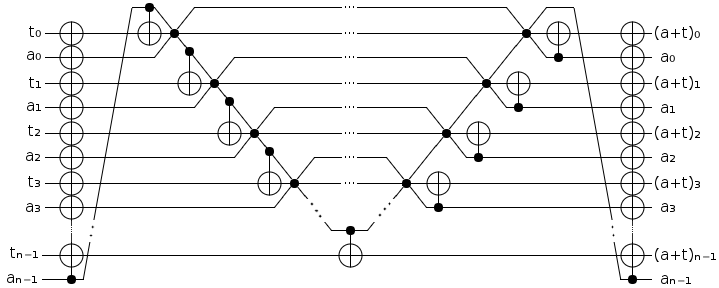
\includegraphics[totalheight=3cm]{inline-adder.png}
  \caption{\em Adder for input and target registers of the same size.
  Requires no ancilla, and uses $O(N)$ gates and depth.
  Based on \cite{van2004, takahashi2005}.}
  \label{fig:inlineadder}
\end{figure}

To perform subtraction instead of addition: run the circuit in reverse, temporarily invert the target register by bordering the circuit with NOT gates on the target, or invert the CSWAP controls.

Because this adder construction uses the input register as workspace, it only works when the input register is the same size as the target register.
When the input register is larger the high bits of the input register can simply be ignored, but when the target register is larger the workaround is more difficult.
Not only is there insufficient workspace, but the register sizes being different breaks the logical-negation trick that allowed the ancilla to be dirty.

To work around the target register being larger, three fixes are needed.
Each uses a controlled increment or decrement gate, which will be described in the next section.
(Note that, to avoid cyclic dependencies, the increment and decrement constructions will only use the same-register-size adder.)
First, the carry signal must be forwarded into the high part of the target register with a controlled increment instead of with a CNOT.
Second, to free the MSB of the input register for use as the carry signal, we add it into the target ahead of time with a controlled increment.
Finally, when the MSB is on instead of off its role as carry signal causes an extra increment of the target.
This extra increment is cancelled with a controlled decrement.
See the circuit diagram in figure \ref{fig:inline-adder-into-large} for the complete construction.

\begin{figure}
  \centering
  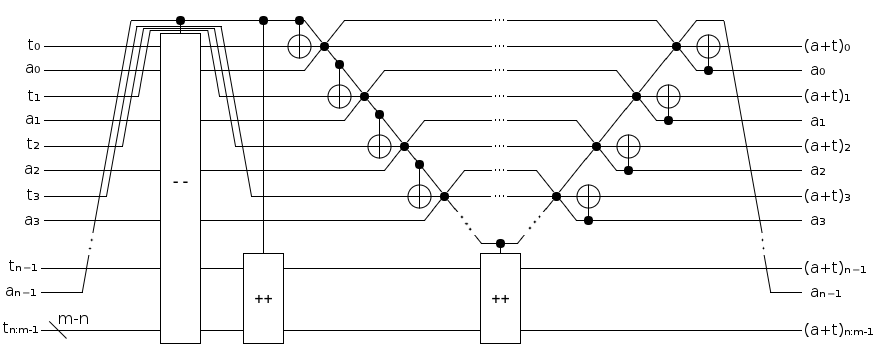
\includegraphics[totalheight=3cm]{inline-adder-into-large.png}
  \caption{\em
      Adder with target larger than source, using no ancilla.
      Uses $O(N)$ gates and depth.
      The increment and decrement gates all have at least one free wire to borrow as a dirty ancilla.}
  \label{fig:inline-adder-into-large}
\end{figure}

\section{$O(N)$ incrementer}

A register can be incremented by subtracting both $x$ and $\neg x = -x-1$ from it, for any $x$.
When $N$ dirty bits are available, $x$ can come from a register defined by those $N$ arbitrary bits, as shown in figure \ref{fig:double-sub-increment}.

\begin{figure}
  \centering
  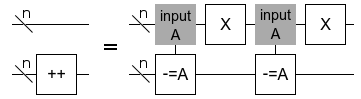
\includegraphics[totalheight=2cm]{double-sub-increment.png}
  \caption{\em Subtracting $x$ and $-x-1$ from a register increments it. Requires $O(N)$ depth, size, and $N$ dirty ancilla.}
  \label{fig:double-sub-increment}
\end{figure}

To improve from $N$ dirty bits to a single dirty bit, we break the increment operation into two halves.
A top half that is incremented only if all of the bottom bits are on, and a bottom half that is unconditionally incremented.
The bottom half can be incremented with the double-subtraction trick by borrowing the top half.
But the double-subtraction trick doesn't work on the top half, because the bottom half can't be borrowed when it is being used as a control.

To work around not being able to operate on the borrowed bits while using them as a control, start with the double-subtraction trick but change the second subtraction to an addition and conditionally toggle the target bits instead of the input bits.
When the condition isn't satisfied, the addition and subtraction will cancel each other.
When the condition is satisfied, the addition will be inverted into a subtraction, and both the subtraction and addition-turned-subtraction will fire, subtracting the input register from the target register twice.
However, because we are conditioning on the input bits all being on, we know the input must be -1.
Therefore the target was incremented by 2.
To halve the +2 into a +1, prepend a dirty LSB onto the target register as shown in \ref{fig:compact-increment}.

\begin{figure}
  \centering
  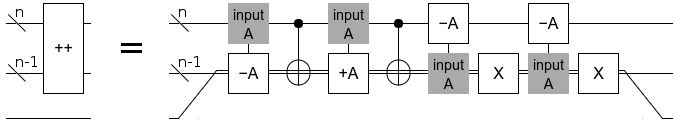
\includegraphics[totalheight=1.5cm]{compact-increment.png}
  \caption{\em Odd-sized $O(N)$ increment with 1 dirty ancilla.}
  \label{fig:compact-increment}
\end{figure}

Because the adder/subtracter construction used by the incrementer in figure \ref{fig:compact-increment} requires the target and source registers to be the same size, the construction described so far only works on odd-sized registers.
For even-sized registers, another minor variation on the conditionally-invert-addition-into-subtraction-with-logical-negation technique is used.
That construction is shown in figure \ref{fig:compact-increment-even}.

\begin{figure}
  \centering
  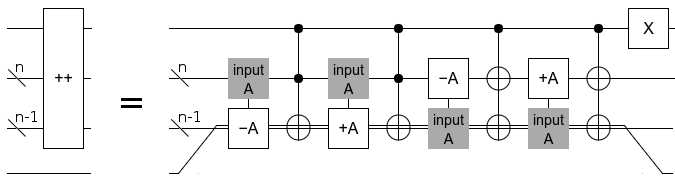
\includegraphics[totalheight=2cm]{compact-increment-even.png}
  \caption{\em Even-sized $O(N)$ increment with 1 dirty ancilla.}
  \label{fig:compact-increment-even}
\end{figure}

As with addition and subtraction, you can turn an increment into a decrement either by reversing the gate order, by bordering the circuit with NOT gates, or by inverting all of the controls.
Also, increment gates can be efficiently controlled by using another invert-input-and-output trick (see figures \ref{fig:controlled-increment-odd} and \ref{fig:controlled-increment-even}).

\begin{figure}
  \centering
  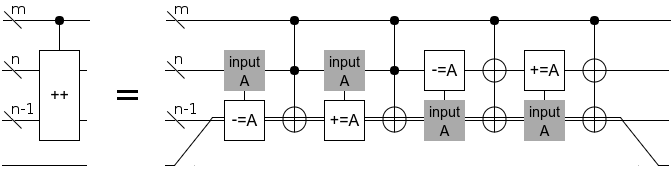
\includegraphics[totalheight=2cm]{controlled-increment-odd.png}
  \caption{\em Odd-sized $O(N)$ controlled increment with 1 dirty ancilla.}
  \label{fig:controlled-increment-odd}
\end{figure}

\begin{figure}
  \centering
  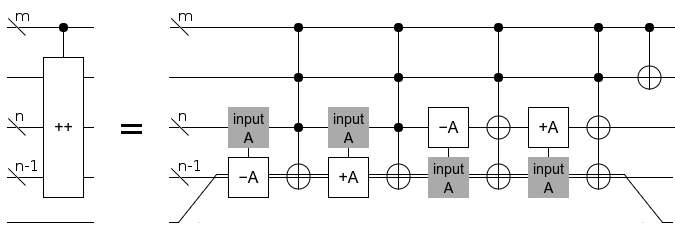
\includegraphics[totalheight=2.5cm]{controlled-increment-even.png}
  \caption{\em Even-sized $O(N)$ controlled increment with 1 dirty ancilla.}
  \label{fig:controlled-increment-even}
\end{figure}

Note that it is impossible to create a classical incrementer that uses no ancilla.
The parity of the permutation performed by an increment operation is odd, but the parity of the permutation performed by any classical gate that doesn't cover the entire circuit is even.
Quantumly, the parity barrier can be bypassed by using partial rotations (see figure \ref{fig:bootstrap-ancilla}).

\begin{figure}
  \centering
  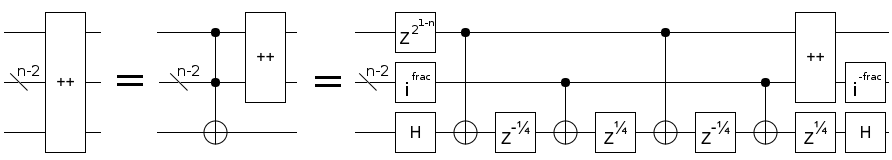
\includegraphics[totalheight=1.4cm]{ancilla-bootstrap.png}
  \caption{\em Bootstrapping a dirty ancilla out of an increment gate using quantum operations.
  The $i^{\text{frac}}$ gate is a ``phase gradient" operation that phases each computational basis state $|v\rangle$ by an amount proportional to $v/2^d$, where $d$ is the size of the register.
  In this case each state is phased by $e^{i \frac{\pi}{2} v/2^d}$.
  The phase gradient is implemented by a column of $Z^{2^{-k}}$ gates, .}
  \label{fig:bootstrap-ancilla}
\end{figure}

\section{$O(N)$ inline comparisons}

We review how to implement comparison operations, which toggle a target bit based on the relationship between two input registers, using addition and subtraction operations.

The is-B-less-than-A comparison is implemented by subtracting $A$ out of $B$, with a target bit appended as $B$'s MSB, then adding $A$ into $B$ without the target bit appended.
See figure \ref{fig:comparison-less}.

\begin{figure}
  \centering
  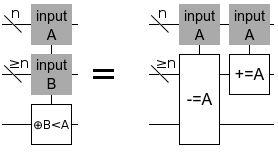
\includegraphics[totalheight=3cm]{comparison-less.png}
  \caption{\em Toggling a target bit if one register is less than another, without using ancilla.}
  \label{fig:comparison-less}
\end{figure}

The same idea is used for is-B-less-than-or-equal-to-A, except $A+1$ is subtracted and added instead of $A$.
The extra $\pm 1$ can be performed by increment and decrement gates, as shown in figure \ref{fig:comparison-leq}.
When the two registers are the same size, the increment gate can be omitted by inverting the $A$ and $B$ registers during the addition.

$>$ and $\geq$ comparisons are done by performing the corresponding opposite comparison ($\leq$ and $<$ respectively) and inverting the result by toggling the target.

Beware that, when the $B$ register is smaller than the $A$ register, the high bits of $A$ are not accounted for by the subtraction and addition and so the construction breaks.
To fix the problem, swap the roles of A and B (i.e. subtract out of A instead) and use the opposite comparison.
Alternatively, any operations generated by the subtraction or decrement gates that toggle the target bit can be controlled by all of the high bits of $A$ being off (and then, if any of those high bits are on, meaning $A$ must be larger than $B$, toggle the result bit as appropriate for the comparison).

\begin{figure}
  \centering
  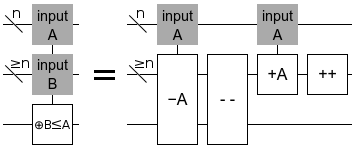
\includegraphics[totalheight=3cm]{comparison-leq.png}
  \caption{\em Toggling a target bit if one register is less than or equal to another, without using ancilla.}
  \label{fig:comparison-leq}
\end{figure}

\section{$\text{PivotFlip}$}

A pivot-flip operation reverses the order of states less than or equal to a given pivot value.
For example, a pivot-flip with the pivot equal to 3 would swap $|0\rangle$ and $|3\rangle$, swap $|1\rangle$ and $|2\rangle$, and leave all other states untouched.
Pivot-flips are useful for implementing cyclic operations, such as modular addition.

The exact permutation performed by a pivot-flip with pivot equal to $k$ is:

$$\text{PivotFlip}_k = \sum_{i=0}^k |k-i\rangle \langle i| + \sum_{i=k+1}^{N-1} |i\rangle \langle i|$$

And the overall permutation, including the pivot input, is:

$$\text{PivotFlip} = \sum_{k=0}^{N-1} |k\rangle \langle k| \otimes \text{PivotFlip}_{k}$$

To perform a pivot-flip efficiently, we use the fact that $x \rightarrow \lnot(x - a - 1)$ nearly does what is required.
As shown in figure \ref{fig:double-flip}, the permutation $x \rightarrow \lnot(x - a - 1)$ flips the range below-and-including the pivot but also flips the range above the pivot.
However, because $x \rightarrow \lnot(x - a - 1)$ is its own inverse and doesn't change whether any value is less than or equal to the pivot, the operation can be controlled by dirty comparisons against the pivot.

By applying $x \rightarrow \lnot(x - a - 1)$ twice, controlled by a dirty bit that is toggled by the comparison, the desired effect is achieved.
For states that are less than or equal to the pivot $a$, the dirty ancilla is being toggled and exactly one of the controlled flips will happen.
For other states, the ancilla does not change and so the controlled flip happens no times or two times, undoing itself.
See figure \ref{fig:const-pivot-flip} fot the construction, as well as a variant that only flips values strictly less than the pivot instead of including the pivot.

\begin{figure}
  \centering
  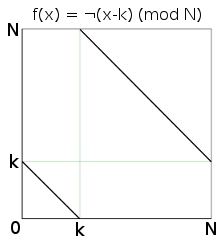
\includegraphics[totalheight=4cm]{double-flip.png}
  \caption{\em Subtraction followed by logical negation performs flips both above and below $k$.}
  \label{fig:double-flip}
\end{figure}

\begin{figure}
  \centering
  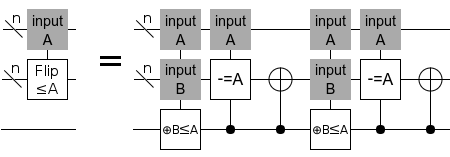
\includegraphics[totalheight=4.5cm]{pivot-flip.png}
  \caption{\em Pivot flip circuits.
  When the top wire bundle is a register, the subtractions are controlled by adding a control to any CNOTs, increments, and decrements in figures \ref{fig:inlineadder} or \ref{fig:inline-adder-into-large}.
  When the top wire bundle is a compile-time constant, the subtractions use the construction from \cite{haner2016} and are controlled as shown in figure \ref{fig:controlled-offset}.}
  \label{fig:const-pivot-flip}
\end{figure}

\begin{figure}
  \centering
  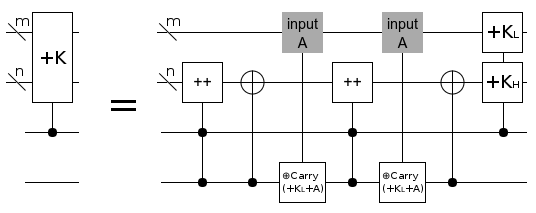
\includegraphics[totalheight=3.1cm]{controlled-offset.png}
  \caption{\em Offset circuit from \cite{haner2016}, modified to include a control.}
  \label{fig:controlled-offset}
\end{figure}

The cost of a $\text{PivotFlip}$ depends on if the pivot is a compile-time constant or not.
When the pivot is input from another register, the $O(N)$ inline adder can be used.
But when the pivot is a constant, the $O(N \lg N)$ size and $O(N)$ depth offset gate from \cite{haner2016} is used instead.

\section{$O(N \lg N)$ Modular Addition and Modular Offset} \label{sec:last-circuit}

A modular addition is three pivot flips.
To add $a$ into a register modulo $r$, perform pivot-flips with the pivot at $r-1-a$, then $r-1$, then $a-1$.
See figure \ref{fig:modular-add}.

Be aware that this construction requires that the input register be in range.
If the input is greater than or equal to $r$, the pivot-flips will trash the target register instead of adding the input mod $r$ into it.

\begin{figure}
  \centering
  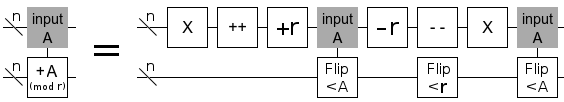
\includegraphics[totalheight=1.4cm]{modular-addition.png}
  \caption{\em Modular addition circuit.
  The $+r$ operations are offset gates requiring $O(N \lg N)$ size when the modulus is a constant.
  The pivot-flips require a dirty bit.}
  \label{fig:modular-add}
\end{figure}

Although the fact is obfuscated by the number of constructions used, our modular addition construction is performed entirely in terms of normal addition (with various tweaks and tricks and inversions along the way).
See figure \ref{fig:modular-dependencies} for the full dependency graph.

The modular addition uses $O(N \lg N)$ gates because that is the cost of the offset gate in \cite{haner2016}, and we subtract the modulus (typically a compile-time constant) out of a register during one of the pivot-flips.
If both the amount to add {\em and the modulus} are in registers, then the construction only requires $O(N)$ gates.
The total depth is $O(N)$ regardless.

\begin{figure}
  \centering
  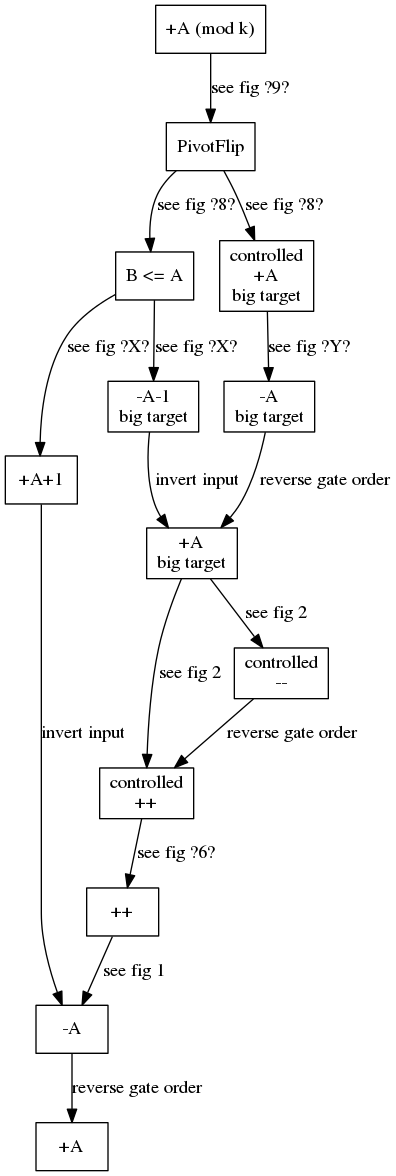
\includegraphics[totalheight=16cm]{modular-add-graph.png}
  \caption{\em
      Dependency graph of constructions used to create a classical reversible modular adder / modular offset gates using only 1 dirty bit.}
  \label{fig:modular-dependencies}
\end{figure}

\section{Factoring with $2n+1$ qubits} \label{sec:applications}

In \cite{haner2016}, H\"{a}ner et al. describe how to perform Shor's algorithm with Toffoli-based circuits using $2n+2$ qubits.
The first $n$ qubits are needed to hold the input.
The second $n$ qubits are for holding the output of exponentiating the input modulo a constant.
One of the remaining qubits is used in the phase estimation process.
The last qubit is a clean ancilla used by their modular offset operation to temporarily hold a comparison against the modulus.

The modular addition circuit we have presented does not require that last clean ancilla.
Instead, we borrow the phase estimation qubit as a temporary dirty bit.
Our modular offset circuit is a drop-in replacement for the one used by H\"{a}ner et all.
It even has the same asymptotic costs: $O(N \lg N)$ size and $O(N)$ depth.
Using our modular offset circuit, and borrowing the phase estimation qubit instead of using a separate clean bit, creates an implementation of Shor's factoring algorithm that uses only $2n+1$ qubits without increasing the size or depth complexity.

\section{Conclusion} \label{sec:conclusion}

We present classical reversible circuits for incrementing, modular addition, and modular offset that use only a single dirty bit.
Our modular offset circuit improves the minimum number of qubits used when factoring an $n$-bit integer from $2n+2$ to $2n+1$.

For incrementing, a single dirty ancilla is classically optimal because the permutation defined by an increment operation is odd.
This obstacle does not apply to modular additions, because any odd parities can made even with a useless swap in the range of states above the modulus.
So it may be possible to elide the final dirty ancilla our modular addition construction requires, even when restricted to Toffoli-based circuits.

\bibliographystyle{plain}
\bibliography{citations}

\section{Temporary Test Circuit Links}

Convenience links for myself when checking that things work.

\href
{http://algassert.com/quirk#circuit=%7B%22cols%22%3A%5B%5B%22X%22%2C%22X%22%2C%22X%22%2C%22X%22%2C%22%E2%80%A2%22%2C%22X%22%2C%22X%22%2C%22X%22%2C%22X%22%2C%22X%22%5D%2C%5B%22%E2%80%A2%22%2C1%2C1%2C1%2C1%2C%22X%22%5D%2C%5B%22Swap%22%2C1%2C1%2C1%2C%22Swap%22%2C%22%E2%80%A2%22%5D%2C%5B1%2C%22%E2%80%A2%22%2C1%2C1%2C1%2C1%2C%22X%22%5D%2C%5B1%2C%22Swap%22%2C1%2C1%2C%22Swap%22%2C1%2C%22%E2%80%A2%22%5D%2C%5B1%2C1%2C%22%E2%80%A2%22%2C1%2C1%2C1%2C1%2C%22X%22%5D%2C%5B1%2C1%2C%22Swap%22%2C1%2C%22Swap%22%2C1%2C1%2C%22%E2%80%A2%22%5D%2C%5B1%2C1%2C1%2C%22%E2%80%A2%22%2C1%2C1%2C1%2C1%2C%22X%22%5D%2C%5B1%2C1%2C1%2C%22Swap%22%2C%22Swap%22%2C1%2C1%2C1%2C%22%E2%80%A2%22%5D%2C%5B1%2C1%2C1%2C1%2C%22%E2%80%A2%22%2C1%2C1%2C1%2C1%2C%22X%22%5D%2C%5B1%2C1%2C1%2C%22Swap%22%2C%22Swap%22%2C1%2C1%2C1%2C%22%E2%80%A2%22%5D%2C%5B1%2C1%2C1%2C1%2C%22%E2%80%A2%22%2C1%2C1%2C1%2C%22X%22%5D%2C%5B1%2C1%2C%22Swap%22%2C1%2C%22Swap%22%2C1%2C1%2C%22%E2%80%A2%22%5D%2C%5B1%2C1%2C1%2C1%2C%22%E2%80%A2%22%2C1%2C1%2C%22X%22%5D%2C%5B1%2C%22Swap%22%2C1%2C1%2C%22Swap%22%2C1%2C%22%E2%80%A2%22%5D%2C%5B1%2C1%2C1%2C1%2C%22%E2%80%A2%22%2C1%2C%22X%22%5D%2C%5B%22Swap%22%2C1%2C1%2C1%2C%22Swap%22%2C%22%E2%80%A2%22%5D%2C%5B1%2C1%2C1%2C1%2C%22%E2%80%A2%22%2C%22X%22%5D%2C%5B%22X%22%2C%22X%22%2C%22X%22%2C%22X%22%2C%22%E2%80%A2%22%2C%22X%22%2C%22X%22%2C%22X%22%2C%22X%22%2C%22X%22%5D%5D%7D}
{5+5-bit inline adder}
(or \href
{http://algassert.com/quirk#circuit=%7B%22cols%22%3A%5B%5B%22Counting10%22%5D%2C%5B%22QFT7%22%5D%2C%5B1%2C1%2C1%2C%22QFT7%22%5D%2C%5B%22%E2%80%A6%22%5D%2C%5B%22%E2%80%A6%22%5D%2C%5B%22X%22%2C%22X%22%2C%22X%22%2C%22X%22%2C%22%E2%80%A2%22%2C%22X%22%2C%22X%22%2C%22X%22%2C%22X%22%2C%22X%22%5D%2C%5B%22%E2%80%A2%22%2C1%2C1%2C1%2C1%2C%22X%22%5D%2C%5B%22Swap%22%2C1%2C1%2C1%2C%22Swap%22%2C%22%E2%80%A2%22%5D%2C%5B1%2C%22%E2%80%A2%22%2C1%2C1%2C1%2C1%2C%22X%22%5D%2C%5B1%2C%22Swap%22%2C1%2C1%2C%22Swap%22%2C1%2C%22%E2%80%A2%22%5D%2C%5B1%2C1%2C%22%E2%80%A2%22%2C1%2C1%2C1%2C1%2C%22X%22%5D%2C%5B1%2C1%2C%22Swap%22%2C1%2C%22Swap%22%2C1%2C1%2C%22%E2%80%A2%22%5D%2C%5B1%2C1%2C1%2C%22%E2%80%A2%22%2C1%2C1%2C1%2C1%2C%22X%22%5D%2C%5B1%2C1%2C1%2C%22Swap%22%2C%22Swap%22%2C1%2C1%2C1%2C%22%E2%80%A2%22%5D%2C%5B1%2C1%2C1%2C1%2C%22%E2%80%A2%22%2C1%2C1%2C1%2C1%2C%22X%22%5D%2C%5B1%2C1%2C1%2C%22Swap%22%2C%22Swap%22%2C1%2C1%2C1%2C%22%E2%80%A2%22%5D%2C%5B1%2C1%2C1%2C1%2C%22%E2%80%A2%22%2C1%2C1%2C1%2C%22X%22%5D%2C%5B1%2C1%2C%22Swap%22%2C1%2C%22Swap%22%2C1%2C1%2C%22%E2%80%A2%22%5D%2C%5B1%2C1%2C1%2C1%2C%22%E2%80%A2%22%2C1%2C1%2C%22X%22%5D%2C%5B1%2C%22Swap%22%2C1%2C1%2C%22Swap%22%2C1%2C%22%E2%80%A2%22%5D%2C%5B1%2C1%2C1%2C1%2C%22%E2%80%A2%22%2C1%2C%22X%22%5D%2C%5B%22Swap%22%2C1%2C1%2C1%2C%22Swap%22%2C%22%E2%80%A2%22%5D%2C%5B1%2C1%2C1%2C1%2C%22%E2%80%A2%22%2C%22X%22%5D%2C%5B%22X%22%2C%22X%22%2C%22X%22%2C%22X%22%2C%22%E2%80%A2%22%2C%22X%22%2C%22X%22%2C%22X%22%2C%22X%22%2C%22X%22%5D%2C%5B%22%E2%80%A6%22%5D%2C%5B%22%E2%80%A6%22%5D%2C%5B%22inputA5%22%2C1%2C1%2C1%2C1%2C%22%2B%3DA5%22%5D%2C%5B1%2C1%2C1%2C%22QFT%E2%80%A07%22%5D%2C%5B%22QFT%E2%80%A07%22%5D%2C%5B%22Uncounting10%22%5D%5D%7D}
{with test harness})

\href
{http://algassert.com/quirk#circuit=%7B%22cols%22%3A%5B%5B%22inputA4%22%2C1%2C1%2C1%2C%22-%3DA4%22%5D%2C%5B%22X%22%2C%22X%22%2C%22X%22%2C%22X%22%5D%2C%5B%22inputA4%22%2C1%2C1%2C1%2C%22-%3DA4%22%5D%2C%5B%22X%22%2C%22X%22%2C%22X%22%2C%22X%22%5D%5D%7D}
{4-bit incrementer w/ 4 dirty}

\href
{http://algorithmicassertions.com/quirk#circuit=%7B%22cols%22%3A%5B%5B1%2C1%2C1%2C1%2C1%2C%22%3C%3C4%22%5D%2C%5B1%2C%22inputA4%22%2C1%2C1%2C1%2C%22-%3DA4%22%5D%2C%5B%22%E2%80%A2%22%2C%22%E2%80%A2%22%2C%22%E2%80%A2%22%2C%22%E2%80%A2%22%2C%22%E2%80%A2%22%2C%22X%22%2C%22X%22%2C%22X%22%2C%22X%22%5D%2C%5B1%2C%22inputA4%22%2C1%2C1%2C1%2C%22%2B%3DA4%22%5D%2C%5B%22%E2%80%A2%22%2C%22%E2%80%A2%22%2C%22%E2%80%A2%22%2C%22%E2%80%A2%22%2C%22%E2%80%A2%22%2C%22X%22%2C%22X%22%2C%22X%22%2C%22X%22%5D%2C%5B1%2C%22-%3DA4%22%2C1%2C1%2C1%2C%22inputA4%22%5D%2C%5B%22%E2%80%A2%22%2C%22X%22%2C%22X%22%2C%22X%22%2C%22X%22%2C%22X%22%2C%22X%22%2C%22X%22%2C%22X%22%5D%2C%5B1%2C%22%2B%3DA4%22%2C1%2C1%2C1%2C%22inputA4%22%5D%2C%5B%22%E2%80%A2%22%2C%22X%22%2C%22X%22%2C%22X%22%2C%22X%22%2C%22X%22%2C%22X%22%2C%22X%22%2C%22X%22%5D%2C%5B%22X%22%5D%2C%5B1%2C1%2C1%2C1%2C1%2C%22%3E%3E4%22%5D%5D%7D}
{8-bit incrementer w/ 1 dirty}
(or \href
{http://algorithmicassertions.com/quirk#circuit=%7B%22cols%22%3A%5B%5B%22Counting9%22%5D%2C%5B%22QFT6%22%5D%2C%5B1%2C1%2C1%2C%22QFT6%22%5D%2C%5B%22%E2%80%A6%22%5D%2C%5B%22%E2%80%A6%22%5D%2C%5B1%2C1%2C1%2C1%2C1%2C%22%3C%3C4%22%5D%2C%5B1%2C%22inputA4%22%2C1%2C1%2C1%2C%22-%3DA4%22%5D%2C%5B%22%E2%80%A2%22%2C%22%E2%80%A2%22%2C%22%E2%80%A2%22%2C%22%E2%80%A2%22%2C%22%E2%80%A2%22%2C%22X%22%2C%22X%22%2C%22X%22%2C%22X%22%5D%2C%5B1%2C%22inputA4%22%2C1%2C1%2C1%2C%22%2B%3DA4%22%5D%2C%5B%22%E2%80%A2%22%2C%22%E2%80%A2%22%2C%22%E2%80%A2%22%2C%22%E2%80%A2%22%2C%22%E2%80%A2%22%2C%22X%22%2C%22X%22%2C%22X%22%2C%22X%22%5D%2C%5B1%2C%22-%3DA4%22%2C1%2C1%2C1%2C%22inputA4%22%5D%2C%5B%22%E2%80%A2%22%2C%22X%22%2C%22X%22%2C%22X%22%2C%22X%22%2C%22X%22%2C%22X%22%2C%22X%22%2C%22X%22%5D%2C%5B1%2C%22%2B%3DA4%22%2C1%2C1%2C1%2C%22inputA4%22%5D%2C%5B%22%E2%80%A2%22%2C%22X%22%2C%22X%22%2C%22X%22%2C%22X%22%2C%22X%22%2C%22X%22%2C%22X%22%2C%22X%22%5D%2C%5B%22X%22%5D%2C%5B1%2C1%2C1%2C1%2C1%2C%22%3E%3E4%22%5D%2C%5B%22%E2%80%A6%22%5D%2C%5B%22%E2%80%A6%22%5D%2C%5B%22dec8%22%5D%2C%5B1%2C1%2C1%2C%22QFT%E2%80%A06%22%5D%2C%5B%22QFT%E2%80%A06%22%5D%2C%5B%22Uncounting9%22%5D%5D%7D}
{with test harness})

\href
{http://algorithmicassertions.com/quirk#circuit=%7B%22cols%22%3A%5B%5B1%2C1%2C1%2C1%2C1%2C%22%3C%3C5%22%5D%2C%5B%22inputA5%22%2C1%2C1%2C1%2C1%2C%22-%3DA5%22%5D%2C%5B%22%E2%80%A2%22%2C%22%E2%80%A2%22%2C%22%E2%80%A2%22%2C%22%E2%80%A2%22%2C%22%E2%80%A2%22%2C%22X%22%2C%22X%22%2C%22X%22%2C%22X%22%2C%22X%22%5D%2C%5B%22inputA5%22%2C1%2C1%2C1%2C1%2C%22%2B%3DA5%22%5D%2C%5B%22%E2%80%A2%22%2C%22%E2%80%A2%22%2C%22%E2%80%A2%22%2C%22%E2%80%A2%22%2C%22%E2%80%A2%22%2C%22X%22%2C%22X%22%2C%22X%22%2C%22X%22%2C%22X%22%5D%2C%5B%22-%3DA5%22%2C1%2C1%2C1%2C1%2C%22inputA5%22%5D%2C%5B1%2C1%2C1%2C1%2C1%2C%22X%22%2C%22X%22%2C%22X%22%2C%22X%22%2C%22X%22%5D%2C%5B%22-%3DA5%22%2C1%2C1%2C1%2C1%2C%22inputA5%22%5D%2C%5B1%2C1%2C1%2C1%2C1%2C%22X%22%2C%22X%22%2C%22X%22%2C%22X%22%2C%22X%22%5D%2C%5B1%2C1%2C1%2C1%2C1%2C%22%3E%3E5%22%5D%5D%7D}
{9-bit incrementer w/ 1 dirty}
(or \href
{http://algorithmicassertions.com/quirk#circuit=%7B%22cols%22%3A%5B%5B%22Counting10%22%5D%2C%5B%22QFT7%22%5D%2C%5B1%2C1%2C1%2C%22QFT7%22%5D%2C%5B%22%E2%80%A6%22%5D%2C%5B%22%E2%80%A6%22%5D%2C%5B1%2C1%2C1%2C1%2C1%2C%22%3C%3C5%22%5D%2C%5B%22inputA5%22%2C1%2C1%2C1%2C1%2C%22-%3DA5%22%5D%2C%5B%22%E2%80%A2%22%2C%22%E2%80%A2%22%2C%22%E2%80%A2%22%2C%22%E2%80%A2%22%2C%22%E2%80%A2%22%2C%22X%22%2C%22X%22%2C%22X%22%2C%22X%22%2C%22X%22%5D%2C%5B%22inputA5%22%2C1%2C1%2C1%2C1%2C%22%2B%3DA5%22%5D%2C%5B%22%E2%80%A2%22%2C%22%E2%80%A2%22%2C%22%E2%80%A2%22%2C%22%E2%80%A2%22%2C%22%E2%80%A2%22%2C%22X%22%2C%22X%22%2C%22X%22%2C%22X%22%2C%22X%22%5D%2C%5B%22-%3DA5%22%2C1%2C1%2C1%2C1%2C%22inputA5%22%5D%2C%5B1%2C1%2C1%2C1%2C1%2C%22X%22%2C%22X%22%2C%22X%22%2C%22X%22%2C%22X%22%5D%2C%5B%22-%3DA5%22%2C1%2C1%2C1%2C1%2C%22inputA5%22%5D%2C%5B1%2C1%2C1%2C1%2C1%2C%22X%22%2C%22X%22%2C%22X%22%2C%22X%22%2C%22X%22%5D%2C%5B1%2C1%2C1%2C1%2C1%2C%22%3E%3E5%22%5D%2C%5B%22%E2%80%A6%22%5D%2C%5B%22%E2%80%A6%22%5D%2C%5B%22dec9%22%5D%2C%5B1%2C1%2C1%2C%22QFT%E2%80%A07%22%5D%2C%5B%22QFT%E2%80%A07%22%5D%2C%5B%22Uncounting10%22%5D%5D%7D}
{with test harness})

\href
{http://algorithmicassertions.com/quirk#circuit=%7B%22cols%22%3A%5B%5B%22Z%5E%E2%85%9F%E2%82%81%E2%82%86%22%2C%22Z%5E%E2%85%9F%E2%82%81%E2%82%86%22%2C%22Z%5E%E2%85%9B%22%2C%22Z%5E%C2%BC%22%2C%22H%22%5D%2C%5B%22%E2%80%A2%22%2C1%2C1%2C1%2C%22X%22%5D%2C%5B1%2C1%2C1%2C1%2C%22Z%5E-%C2%BC%22%5D%2C%5B1%2C%22%E2%80%A2%22%2C%22%E2%80%A2%22%2C%22%E2%80%A2%22%2C%22X%22%5D%2C%5B1%2C1%2C1%2C1%2C%22Z%5E%C2%BC%22%5D%2C%5B%22%E2%80%A2%22%2C1%2C1%2C1%2C%22X%22%5D%2C%5B1%2C1%2C1%2C1%2C%22Z%5E-%C2%BC%22%5D%2C%5B1%2C%22%E2%80%A2%22%2C%22%E2%80%A2%22%2C%22%E2%80%A2%22%2C%22X%22%5D%2C%5B%22inc4%22%2C1%2C1%2C1%2C%22Z%5E%C2%BC%22%5D%2C%5B1%2C%22Z%5E-%E2%85%9F%E2%82%81%E2%82%86%22%2C%22Z%5E-%E2%85%9B%22%2C%22Z%5E-%C2%BC%22%2C%22H%22%5D%5D%7D}
{Quantum incrementer ancilla bootstrap}

NOTE: have to open these next ones against local version, because online version doesn't have the comparison gates

\href
{http://algassert.com/quirk#circuit=%7B%22cols%22%3A%5B%5B%22inputA4%22%2C1%2C1%2C1%2C%22inputB4%22%2C1%2C1%2C1%2C%22%5EA%3EB%22%5D%2C%5B%22inputA4%22%2C1%2C1%2C1%2C%22-%3DA4%22%2C1%2C1%2C1%2C%22%E2%80%A2%22%5D%2C%5B1%2C1%2C1%2C1%2C%22X%22%2C%22X%22%2C%22X%22%2C%22X%22%2C%22%E2%80%A2%22%5D%2C%5B%22inputA4%22%2C1%2C1%2C1%2C%22inputB4%22%2C1%2C1%2C1%2C%22%5EA%3EB%22%5D%2C%5B%22inputA4%22%2C1%2C1%2C1%2C%22-%3DA4%22%2C1%2C1%2C1%2C%22%E2%80%A2%22%5D%2C%5B1%2C1%2C1%2C1%2C%22X%22%2C%22X%22%2C%22X%22%2C%22X%22%2C%22%E2%80%A2%22%5D%5D%7D}
{4+4-Bit $<$ PivotFlip}
(or \href
{http://algassert.com/quirk#circuit=%7B%22cols%22%3A%5B%5B1%2C1%2C1%2C1%2C%22H%22%2C%22H%22%2C%22H%22%2C%22H%22%5D%2C%5B%22Counting4%22%2C1%2C1%2C1%2C%22inputA4%22%2C1%2C1%2C1%2C%22%2B%3DA4%22%2C1%2C1%2C1%2C%22X%5Et%22%5D%2C%5B1%2C1%2C1%2C1%2C1%2C1%2C1%2C1%2C%22%3C%3C5%22%5D%2C%5B%22%E2%80%A6%22%5D%2C%5B%22%E2%80%A6%22%5D%2C%5B%22inputA4%22%2C1%2C1%2C1%2C%22inputB4%22%2C1%2C1%2C1%2C%22%5EA%3EB%22%5D%2C%5B%22inputA4%22%2C1%2C1%2C1%2C%22-%3DA4%22%2C1%2C1%2C1%2C%22%E2%80%A2%22%5D%2C%5B1%2C1%2C1%2C1%2C%22X%22%2C%22X%22%2C%22X%22%2C%22X%22%2C%22%E2%80%A2%22%5D%2C%5B%22inputA4%22%2C1%2C1%2C1%2C%22inputB4%22%2C1%2C1%2C1%2C%22%5EA%3EB%22%5D%2C%5B%22inputA4%22%2C1%2C1%2C1%2C%22-%3DA4%22%2C1%2C1%2C1%2C%22%E2%80%A2%22%5D%2C%5B1%2C1%2C1%2C1%2C%22X%22%2C%22X%22%2C%22X%22%2C%22X%22%2C%22%E2%80%A2%22%5D%2C%5B%22%E2%80%A6%22%5D%2C%5B%22%E2%80%A6%22%5D%2C%5B1%2C1%2C1%2C1%2C1%2C1%2C1%2C1%2C%22%3E%3E5%22%5D%2C%5B1%2C1%2C1%2C1%2C1%2C1%2C1%2C1%2C1%2C1%2C1%2C1%2C%22X%5E-t%22%5D%2C%5B%22Chance4%22%2C1%2C1%2C1%2C%22Amps8%22%2C1%2C1%2C1%2C1%2C1%2C1%2C1%2C%22Chance%22%5D%5D%7D}
{with test harness})

\href
{http://algassert.com/quirk#circuit=%7B%22cols%22%3A%5B%5B%22inputA4%22%2C1%2C1%2C1%2C%22inputB4%22%2C1%2C1%2C1%2C%22%5EA%3E%3DB%22%5D%2C%5B%22inputA4%22%2C1%2C1%2C1%2C%22-%3DA4%22%2C1%2C1%2C1%2C%22%E2%80%A2%22%5D%2C%5B1%2C1%2C1%2C1%2C%22dec4%22%2C1%2C1%2C1%2C%22%E2%80%A2%22%5D%2C%5B1%2C1%2C1%2C1%2C%22X%22%2C%22X%22%2C%22X%22%2C%22X%22%2C%22%E2%80%A2%22%5D%2C%5B%22inputA4%22%2C1%2C1%2C1%2C%22inputB4%22%2C1%2C1%2C1%2C%22%5EA%3E%3DB%22%5D%2C%5B%22inputA4%22%2C1%2C1%2C1%2C%22-%3DA4%22%2C1%2C1%2C1%2C%22%E2%80%A2%22%5D%2C%5B1%2C1%2C1%2C1%2C%22dec4%22%2C1%2C1%2C1%2C%22%E2%80%A2%22%5D%2C%5B1%2C1%2C1%2C1%2C%22X%22%2C%22X%22%2C%22X%22%2C%22X%22%2C%22%E2%80%A2%22%5D%5D%7D}
{4+4-Bit $\leq$ PivotFlip}
(or \href
{http://algassert.com/quirk#circuit=%7B%22cols%22%3A%5B%5B1%2C1%2C1%2C1%2C%22H%22%2C%22H%22%2C%22H%22%2C%22H%22%5D%2C%5B%22Counting4%22%2C1%2C1%2C1%2C%22inputA4%22%2C1%2C1%2C1%2C%22%2B%3DA4%22%2C1%2C1%2C1%2C%22X%5Et%22%5D%2C%5B1%2C1%2C1%2C1%2C1%2C1%2C1%2C1%2C%22%3C%3C5%22%5D%2C%5B%22%E2%80%A6%22%5D%2C%5B%22%E2%80%A6%22%5D%2C%5B%22inputA4%22%2C1%2C1%2C1%2C%22inputB4%22%2C1%2C1%2C1%2C%22%5EA%3E%3DB%22%5D%2C%5B%22inputA4%22%2C1%2C1%2C1%2C%22-%3DA4%22%2C1%2C1%2C1%2C%22%E2%80%A2%22%5D%2C%5B1%2C1%2C1%2C1%2C%22dec4%22%2C1%2C1%2C1%2C%22%E2%80%A2%22%5D%2C%5B1%2C1%2C1%2C1%2C%22X%22%2C%22X%22%2C%22X%22%2C%22X%22%2C%22%E2%80%A2%22%5D%2C%5B%22inputA4%22%2C1%2C1%2C1%2C%22inputB4%22%2C1%2C1%2C1%2C%22%5EA%3E%3DB%22%5D%2C%5B%22inputA4%22%2C1%2C1%2C1%2C%22-%3DA4%22%2C1%2C1%2C1%2C%22%E2%80%A2%22%5D%2C%5B1%2C1%2C1%2C1%2C%22dec4%22%2C1%2C1%2C1%2C%22%E2%80%A2%22%5D%2C%5B1%2C1%2C1%2C1%2C%22X%22%2C%22X%22%2C%22X%22%2C%22X%22%2C%22%E2%80%A2%22%5D%2C%5B%22%E2%80%A6%22%5D%2C%5B%22%E2%80%A6%22%5D%2C%5B1%2C1%2C1%2C1%2C1%2C1%2C1%2C1%2C%22%3E%3E5%22%5D%2C%5B1%2C1%2C1%2C1%2C1%2C1%2C1%2C1%2C1%2C1%2C1%2C1%2C%22X%5E-t%22%5D%2C%5B%22Chance4%22%2C1%2C1%2C1%2C%22Amps8%22%2C1%2C1%2C1%2C1%2C1%2C1%2C1%2C%22Chance%22%5D%5D%7D}
{with test harness})

\href
{http://algassert.com/quirk#circuit=%7B%22cols%22%3A%5B%5B1%2C1%2C1%2C1%2C1%2C1%2C1%2C1%2C%22inc4%22%5D%2C%5B%22X%22%2C1%2C1%2C%22X%22%2C%22Counting4%22%2C1%2C1%2C1%2C%22QFT4%22%5D%2C%5B1%2C1%2C1%2C1%2C1%2C1%2C1%2C1%2C%22inputA4%22%2C1%2C1%2C1%2C%22%2B%3DA4%22%5D%2C%5B%22Chance4%22%2C1%2C1%2C1%2C%22Chance4%22%2C1%2C1%2C1%2C%22Chance4%22%5D%2C%5B%22%E2%80%A6%22%5D%2C%5B%22%E2%80%A6%22%5D%2C%5B%22inputA4%22%2C1%2C1%2C1%2C%22%2B%3DA4%22%5D%2C%5B1%2C1%2C1%2C1%2C%22X%22%2C%22X%22%2C%22X%22%2C%22X%22%5D%2C%5B1%2C1%2C1%2C1%2C%22inc4%22%5D%2C%5B1%2C1%2C1%2C1%2C%22inputA4%22%2C1%2C1%2C1%2C%22Flip%3CA4%22%5D%2C%5B1%2C1%2C1%2C1%2C%22dec4%22%5D%2C%5B1%2C1%2C1%2C1%2C%22X%22%2C%22X%22%2C%22X%22%2C%22X%22%5D%2C%5B%22inputA4%22%2C1%2C1%2C1%2C1%2C1%2C1%2C1%2C%22Flip%3CA4%22%5D%2C%5B%22inputA4%22%2C1%2C1%2C1%2C%22%2B%3DA4%22%5D%2C%5B1%2C1%2C1%2C1%2C%22inputA4%22%2C1%2C1%2C1%2C%22Flip%3CA4%22%5D%2C%5B%22%E2%80%A6%22%5D%2C%5B%22%E2%80%A6%22%5D%2C%5B%22Chance4%22%2C1%2C1%2C1%2C%22Chance4%22%2C1%2C1%2C1%2C%22Amps8%22%5D%2C%5B%5D%2C%5B%5D%2C%5B%5D%2C%5B%5D%2C%5B%5D%2C%5B%5D%2C%5B%5D%2C%5B1%2C1%2C1%2C1%2C1%2C1%2C1%2C1%2C%22%7C0%E2%9F%A9%E2%9F%A80%7C%22%5D%2C%5B%22inputB4%22%2C1%2C1%2C1%2C%22inputA4%22%2C1%2C1%2C1%2C%22%5EA%3E%3DB%22%5D%2C%5B1%2C1%2C1%2C1%2C1%2C1%2C1%2C1%2C%22Chance%22%5D%2C%5B1%2C1%2C1%2C1%2C1%2C1%2C1%2C1%2C%22~a82g%22%5D%5D%2C%22gates%22%3A%5B%7B%22id%22%3A%22~a82g%22%2C%22name%22%3A%22IGNORE%22%2C%22matrix%22%3A%22%7B%7B1%2C0%7D%2C%7B0%2C1%7D%7D%22%7D%5D%7D}
{Modular Addition with test Harness}

\end{document}
